% section 2 : activités
\section{Activités du stage}
\subsection{Analyse}
Cette section aborde les informations récoltées pour définir les problèmes à résoudre et les corrections à apporter.
\subsubsection{Les tests sur le système}
Pour connaître les problèmes liés au déploiement de Pharo dans un environnement en lecture seule, j'ai élaboré une liste de tests que j'ai effectués en conditions "normales", c'est-à-dire dans un répertoire où l'écriture est possible, et dans un répertoire en lecture seule. Je passerai en revue ces tests ci-dessous, en spécifiant le comportement observé dans chacun des cas, et les classerai en 3 catégories :
\begin{description}
	\item[Fonctionnement normal :] La fonctionnalité a le comportement attendu, il n'y a rien à corriger.
	\item[Fonctionnement altéré :] La fonctionnalité a un comportement inattendu, mais ne renvoie pas forcément d'erreur.
	\item[Fonctionnement impossible :] La fonctionnalité est inutilisable en l'état, et renvoie systématiquement une erreur.
\end{description}

\paragraph{Le système de log :}
Le log est un mécanisme permettant aux développeurs d'identifier des problèmes lors de l'exécution d'un programme en écrivant la trace de celle-ci dans un fichier. Pour tester ce système, j'ai exécuté la commande suivante :
\begin{verbatim}
Smalltalk logDuring: [ :stream |
                        stream nextPutAll: 'Hello log'; cr ]
\end{verbatim}
Cette commande envoie le message \verb$logDuring:$ à la classe \verb$Smalltalk$, ce qui a pour effet d'exécuter le bloc placé en paramètre en lui donnant accès à un stream vers le fichier de log. Ici, le bloc est le suivant :

\begin{verbatim}
[ :stream | stream nextPutAll: 'Hello log'; cr]
\end{verbatim}

Ce dernier prend un paramètre nommé \verb$stream$ et lui envoie le message \verb$nextPutAll:$ , ce qui écrit dans le stream la chaîne de caractères \verb$'Hello log'$. Puis le message \verb$cr$ est envoyé en cascade pour effectuer un retour chariot. Le résultat attendu est l'apparition du message "Hello log" dans le fichier de log.

Dans des conditions "classiques", le message est correctement écrit dans le fichier.

Dans le cas du système Read-Only, il ne se passe rien : aucune erreur n'apparaît, ce qui est un bon point, cependant, en examinant le fichier de log on observe que le message n'est pas écrit. J'ai donc classé ce problème dans la catégorie "Fonctionnement altéré".

\paragraph{Lancement des tests (Test Runner) :}
Pharo, c'est 6499 classes, 86479 méthodes et 13395 tests, ce qui représente beaucoup de travail si on souhaite lancer tous les tests du système. C'est là que le Test Runner trouve tout son intérêt : Ce programme inclus dans Pharo permet de voir et de lancer tous les tests existants avec un interface clair et simple d'utilisation. Son fonctionnement est très intuitif : on sélectionne le ou les paquets à tester dans la colonne de gauche, puis les classes de test dans la colonne de droite. Enfin, on clique sur le bouton correspondant à ce qui nous intéresse, lancement des tests ou couverture du code. On peut ensuite consulter le résultat dans la partie droite de la fenêtre qui indique l'issue des tests lancés avec un code couleur:

\begin{description}
	\item[le fond est vert :] les tests ont tous passé, il n'y a pas de problème.
	\item[le fond est jaune :] il y a des erreurs non-bloquantes, il est conseillé de les corriger.
	\item[le fond est rouge :] il y a des erreurs bloquantes, comme une exception lancée par exemple, il faut corriger au plus vite.
\end{description}

\begin{figure}[h]
	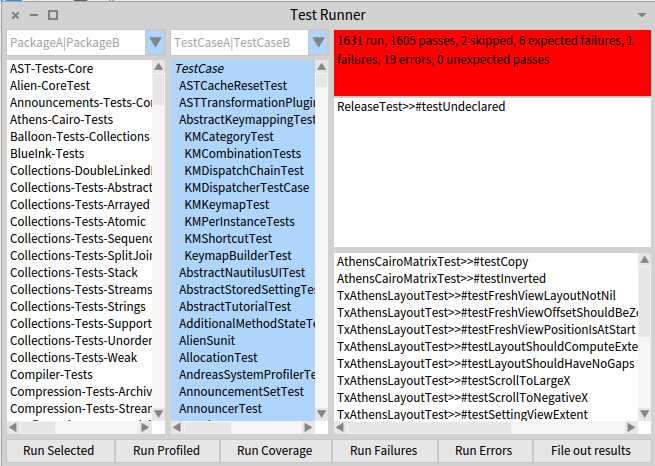
\includegraphics[width=\linewidth]{./img/testrunner.png}
	\caption[testrunner]{Le Test Runner}
\end{figure}

Pour vérifier le fonctionnement du Test Runner, je l'ai ouvert pour lancer tous les tests. Le résultat est bon : il fonctionne aussi bien dans des conditions "normales" qu'en Read-Only, seul le nombre de tests réussis change :
\begin{itemize}
	\item en conditions "normales" : sur 13671 tests lancés, 13599 passent, 26 sont iqnorés, 57 déclenchent une erreur prévue, 7 échouent et 8 erreurs ont étés levées.
	\item en conditions read-only : sur 12620 tests lancés, 11575 passent, 16 sont iqnorés, 87 déclenchent une erreur prévue, 28 échouent et 930 erreurs ont étés levées.
\end{itemize}

Le résultat des tests indique que plusieurs systèmes sont défaillants, mais le Test Runner fonctionne sans problème, je l'ai donc classé dans "Fonctionnement normal".

\paragraph{Écriture de code (Nautilus) :}
Pour écrire du code dans Pharo, on utilise Nautilus, le navigateur du système. Il donne accès aux paquets, classes et méthodes, et permet la modification ainsi que la création de ces derniers. Bien que Nautilus soit amené à être remplacé par Calypso dans Pharo 7, je l'ai tout de même testé pour être complet.

\begin{figure}[h]
	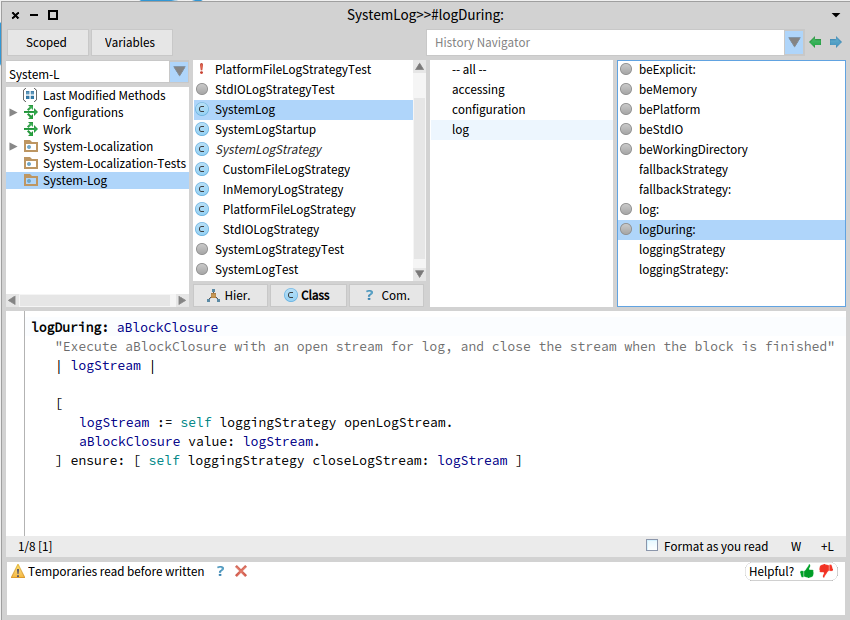
\includegraphics[width=\linewidth]{./img/nautilus.png}
	\caption[nautilus]{Nautilus, le navigateur de Pharo}
\end{figure}

Mon test consistait en la création d'une classe et d'une méthode, et la modification de ces dernières. En conditions "normales", il n'y a aucun problème. En read-only, la création de la classe comme de la méthode provoque l'apparition d'erreurs, mais la création se fait tout de même. La modification d'une méthode fonctionne, mais celle d'une classe freeze l'image.

Il est possible de coder, mais avec des erreurs, je l'ai donc classé dans "Fonctionnement altéré".

\paragraph{La sauvegarde (Monticello) :}
Monticello est un système de contrôle de version (VCS) comme git, c'est-à-dire qu'il permet de sauvegarder les modifications apportées à un moment donné sous forme de commits, permettant ainsi de pouvoir revenir dans le passé via ces derniers. En plus de permettre une sauvegarde en local, Monticello propose de sauvegarder les modifications dans un repository en ligne, via un service comme Smalltalkhub. Monticello est amené à être remplacé dans Pharo 7 par Calypso, un VCS plus centré sur git avec une gestion par repository plutôt que par paquet pour Monticello.

\begin{figure}[h]
	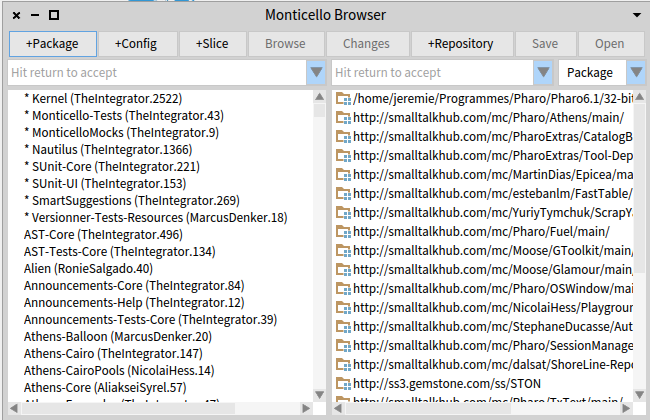
\includegraphics[width=\linewidth]{./img/monticello.png}
	\caption[monticello]{Monticello}
\end{figure}

Le test consistait à enregistrer une modification et à charger un paquet dans Monticello. Si en conditions "normales" la manipulation ne pose aucun problème, il est impossible de sauvegarder en read-only, que ce soit en local ou en ligne. La seule option possible est d'enregistrer dans les fichiers temporaires, ce qui ne permet donc pas de faire une vraie sauvegarde. De plus, tenter un commit renvoit une erreur. Pour le chargement, le résultat est plus radical, car ce dernier provoque un freeze de l'image. J'ai donc classé Monticello dans la catégorie "Fonctionnement impossible".

\paragraph{Le playground :}
Le playground est comme son nom l'indique un bac à sable où l'on exécute du code librement. Servant d'invite de commande, c'est l'un des points d'entrée du système, permettant de lancer un programme, d'imprimer le résultat d'une évaluation et d'analyser la composition d'un objet (un des avantages du système "vivant"), entre autres. Il dispose de plus d'un système d'historique permettant de récupérer le contenu d'une session précédente qui a été fermée par mégarde par exemple.



Mon test visait à tester ce système d'historique en écrivant quelque chose dans le playground avant de le fermer et de tenter dans un autre de récupérer le code écrit. Si cela ne pose aucun problème en conditions "normales", la moindre modification entrée dans le playground (ajout d'un caractère par exemple) déclenchera une erreur non-bloquante, ce qui entrave vraiment l'utilisation du playground, étant obligé d'entrer un caractère et de fermer l'erreur en boucle. De plus, l'historique est indisponible, ce qui place donc le playground dans la catégorie "Fonctionnement impossible".

\paragraph{L'inspecteur :}
La fonction de l'inspecteur est d'afficher la composition d'un objet pour permettre de connaître la valeur de chaque attribut à un moment donné ce qui est très utile quand on cherche à corriger une erreur.

Mon test consistait à vérifier si l'inspecteur peut afficher le contenu d'un objet lambda, par exemple un nombre entier. Si l'inspection ne pose aucun problème en conditions "normales", rien ne s'affiche dans la fenêtre quand on est en lecture seule, déclenchant une erreur au passage. Je l'ai donc classé dans la catégorie "Fonctionnement impossible".

\paragraph{Recherche dans le système (Spotter/senders/implementors) :}
	Le Spotter est un outil de recherche rapide qui affiche tous les résultats (classes, méthodes, paquets, références, ...) correspondant au texte donné, et permettant d'ouvrir le navigateur pour en visualiser le code.
	Pour mieux connaître le fonctionnement d'un algorithme, Pharo permet d'afficher les classes implémentant (implementors) ou appelant (senders) une méthode.
	Pour tester ces fonctionnalités, j'ai cherché une classe avec le Spotter, puis cherché les implémenteurs et les senders d'une méthode, et elles fonctionnent parfaitement bien, que ce soit en conditions "normales" ou en lecture seule, ce qui les classent dans la catégorie "Fonctionnement normal"

\paragraph{Gestion d'erreurs (Debugger) :}
Le debugger Pharo est très performant, car il permet à un développeur de coder au travers de ce dernier : en effet, il suffit d'écrire le message que l'on veut implémenter, l'exécuter, ce qui ouvre le debugger avec une option permettant le cas échéant la création de la méthode/classe manquante, avant de relancer l'exécution là où elle s'était arrêtée. De plus, il affiche la trace des appels et permet de connaître à chacun d'entre eux le contenu de la mémoire pour donner tous les éléments nécessaires à la détection d'une erreur.
Pour tester le debugger, j'ai volontairement déclenché une exception (que je teste au passage de ce fait) pour vérifier si le debugger s'affiche avec la trace, ce qui est le cas quelques soient les conditions. Je le classe donc dans la catégorie "Fonctionnement normal".

\paragraph{Lecture et écriture de fichier :}
Probablement un des points les plus importants de cette série de tests, la lecture et l'écriture de fichier est un des mécanismes les plus importants. Pour les tester, j'ai tenté de lire et d'écrire un fichier dans un répertoire en lecture seule et dans un répertoire inscriptible. 

\subsubsection{Enquête auprès de la communauté}
Avant de commencer à corriger les problèmes identifiés, j'ai fait une enquête (en anglais) auprès de la communauté de Pharo, intitulée "How Pharo should act in a read-only environment ?" (Comment Pharo devrait se comporter dans un environnement en lecture seule ?), pour avoir leur avis sur le comportement que Pharo devrait adopter au terme des réparations. J'ai récolté 25 réponses à cette enquête. Pour chaque question, plusieurs réponses étaient proposées, tout en laissant aux sondés la possibilité de donner une réponse différente si les propositions ne leurs convenaient pas. Ci-dessous sont listées les questions avec la répartition des réponses et une analyse de celles-ci.

\paragraph{1/ Est-ce que les tests qui écrivent dans un fichier devraient être lancés ?}
\subparagraph{Réponses balisées :}
\begin{itemize}
	\item 24\% des sondés se moquent de savoir si les tests sont lancés ou non, car ces derniers n'ont pas été écrit dans le but d'être lancé en lecture seule.
	\item 20\% des sondés souhaitent que les tests soient lancés, mais que ces derniers doivent échouer si le système est en lecture seule.
	\item 12\% des sondés souhaitent que les tests soient lancés et réussissent que ce soit en conditions "normales" ou en lecture seule.
	\item 8\% des sondés ne souhaitent pas que les tests puissent être lancés en lecture seule.
	\item 8\% des sondés ne se prononcent pas.
\end{itemize}

\subparagraph{Réponses libres :}
\begin{itemize}
	\item Certains tests peuvent être modifiés pour fonctionner dans un environnement en lecture seule, mais pas tous. Une solution pourrait être de diviser les tests en 2 catégories : les "vrais" tests unitaires et les tests "pas vraiment" unitaires.
	\item Ces tests devraient être lancés en mémoire ou être ignorés.
	\item Un mock devrait être généré automatiquement.
	\item Pourquoi tester dans un environnement en lecture seule ? Les tests suggèrent du débug, donc de l'écriture de code, donc de l'écriture tout court.
	\item Si un système est fait pour être lancé en lecture seule, il devrait être possible de marquer (avec un pragma par exemple) les tests qui ne devraient pas être lancés et ceux qui devraient l'être (pour permettre de tester le mode read-only).
	\item Il faudrait ajouter une extension pour les tests écrivant dans un fichier et la désactiver quand le système est en lecture seule.
	\item J'aimerai que tous les tests réussissent, mais attendre des tests qu'ils échouent semble plus raisonnable.
\end{itemize}

\subparagraph{Analyse :}
L'idée générale est que les tests devraient pouvoir être lancés, mais qu'ils devraient soit échouer, soit être ignorés. En soit la première option est déjà implémentée, car les tests échouent inévitablement si l'écriture échoue. La catégorisation est une idée intéressante, mais qui demande un travail plus approfondi pour trouver un système qui soit simple d'utilisation tout en assurant que le système ne sera pas trop impacté.

\paragraph{2/ Devrait-il être possible de créer des classes et/ou des méthodes ?}
\subparagraph{Réponses balisées :}
\begin{itemize}
	\item 60\% des sondés souhaitent être capable d'écrire du code sans être confronté à une erreur.
	\item 16\% des sondés considèrent que le système ne devrait pas accepter de changements si il est en lecture seule.
	\item 8\% des sondés souhaite pouvoir écrire du code, quitte à ce que le système lève des exceptions.
	\item 4\% des sondés ne se prononcent pas.
\end{itemize}

\subparagraph{Réponses libres :}
\begin{itemize}
	\item Il devrait être possible de customiser le système avec un script lancé au démarrage pouvant ajouter des classes, etc. Il n'est pas nécessaire de sauvegarder quoi que ce soit.
	\item Plutôt non (car le système est en lecture seule), ou d'une façon non persistante.
	\item Oui, mais uniquement dans la mémoire.
	\item Nous devrions pouvoir le faire, mais sans sauvegarder.
\end{itemize}

\subparagraph{Analyse :}
La majorité des sondés désire pouvoir coder sans problème, tandis qu'une partie un peu plus petite est prête à abandonner la sauvegarde pour pouvoir écrire du code, supposant que lancer Pharo en lecture seule implique de ne pouvoir qu'exécuter du code.

\paragraph{3/ Devrait-il être possible de sauvegarder les changements dans Monticello ?}
\subparagraph{Réponses balisées :}
\begin{itemize}
	\item 40\% des sondés souhaitent que Monticello ignore son package-cache posant problème pour pouvoir le faire fonctionner .
	\item 24\% des sondés ne souhaitent pas pouvoir sauvegarder avec Monticello si le système est en lecture seule.
	\item 12\% des sondés ne se prononcent pas.
	\item 8\% des sondés souhaitent que Monticello écrive son cache dans une zone inscriptible pour qu'il puisse fonctionner normalement.
\end{itemize}

\subparagraph{Réponses libres :}
\begin{itemize}
	\item Monticello pourrait écrire dans /tmp, par exemple
	\item Tout dépends si le package-cache est inscriptible ou non.
	\item Un système read-only devrait le rester.
	\item Il faudrait pouvoir sauvegarder les paquets sur un serveur distant en utilisant git.
\end{itemize}

\subparagraph{Analyse :}
La majorité des sondés souhaitent que Monticello soit fonctionnel, mais ne sont pas tous d'accord sur les modifications à apporter au package-cache, qui est à l'origine de la défaillance. Certains suggèrent que le cache soit purement et simplement ignoré, d'autres que le cache en question soit écrit dans une zone inscriptible.

\paragraph{4/ Devrait-il être possible d'utiliser l'inspecteur ?}
\subparagraph{Réponses balisées :}
\begin{itemize}
	\item 80\% des sondés pensent que oui, car l'inspecteur est une pièce importante de l'IDE.
	\item 8\% des sondés n'ont pas de préférence à ce sujet, car selon eux une application en lecture seule est déjà déployée.
	\item 4\% des sondés ne souhaite pas pouvoir utiliser l'inspecteur en lecture seule.
	\item 4\% des sondés ne se prononcent pas.
\end{itemize}

\subparagraph{Réponses libres :}
\begin{itemize}
	\item Les inspecteurs peuvent faire partie de l'application, qu'elle soit en lecture seule ou non.
\end{itemize}

\subparagraph{Analyse :}
Les résultats pour cette question sont très clair : l'inspecteur doit pouvoir fonctionner en lecture seule de part sa grande utilité dans le développement.

\paragraph{5/ Est-ce que le playground devrait avoir un historique disponible ?}
\subparagraph{Réponses balisées :}
\begin{itemize}
	\item 44\% des sondés pensent que oui, il en faudrait un qui soit sauvegardé dans la mémoire du système.
	\item 28\% des sondés pensent que le playground ne devrait pas en avoir en lecture seule.
	\item 12\% des sondés ne se prononcent pas.
	\item 8\% des sondés pensent qu'il faut un historique écrit dans un répertoire inscriptible.
\end{itemize}

\subparagraph{Réponses libres :}
\begin{itemize}
	\item Il devrait y en avoir un stocké en mémoire, avec la possibilité de définir un fichier pour sauvegarder en utilisant la ligne de commande.
\end{itemize}

\subparagraph{Analyse :}
La majorité des sondés souhaite que le playground puisse avoir un historique quand le système est read-only, avec une préférence pour la sauvegarde en mémoire.

\paragraph{6/ Que devrait-il se passer pour le log du système par défaut ?}
\subparagraph{Réponses balisées :}
\begin{itemize}
	\item 68\% des sondés souhaitent que le log soit écrit dans un emplacement par défaut défini par le système d'exploitation (par exemple /var/log pour Linux).
	\item 12\% des sondés souhaitent que le log soit ignoré.
	\item 8\% des sondés souhaitent que le log soit imprimé dans le terminal.
	\item 4\% des sondés ne se prononcent pas.
\end{itemize}

\subparagraph{Réponses libres :}
\begin{itemize}
	\item Le log devrait être écrit en mémoire, mais avec la possibilité d'utiliser la ligne de commande pour spécifier un fichier destiné au log.
	\item Le log devrait être envoyé à un serveur distant.
\end{itemize}

\subparagraph{Analyse :}
La majorité des sondés désirent avoir du log écrit dans un répertoire du système d'exploitation dédié à cette fonction.

\paragraph{}
La question suivante n'a été posée que si le sondé répondait positivement ou librement à la question 2. 21 personnes sur les 25 ont répondues à cette question

\paragraph{7/ Où devrait être stocké le code par défaut?}
\subparagraph{Réponses balisées :}
\begin{itemize}
	\item 66,7\% des sondés souhaitent que le code soit stocké en mémoire, et qu'il soit donc oublié à la fermeture de Pharo.
	\item 9,5\% des sondés souhaitent que le code soit écrit dans un autre fichier à part.
	\item 9,5\% des sondés souhaitent que le code soit stocké dans une base de données dans un emplacement connu.
	\item 4,8\% des sondés pensent qu'il ne faudrait pas développé dans un système en lecture seule.
\end{itemize}

\subparagraph{Réponses libres :}
\begin{itemize}
	\item Pourquoi le code devrait-il être écrit dans un emplacement inscriptible ? On ne sauvegarde rien quand on est en lecture seule.
\end{itemize}

\subparagraph{Analyse :}
La majorité des sondés souhaitent que le code soit simplement stocké en mémoire. De mon point de vue, cette possibilité permettrait de corriger un bug sans être obligé de réinstaller Pharo après avoir fait la correction dans un autre endroit, que ce soit une autre machine ou un autre répertoire.

%\subsubsection{Problématique}

%\subsection{Conception d'une solution de logging}
%\subsubsection{Architecture}

%\subsubsection{Fonctionnalités}

%\subsubsection{Résolution du problème}

%\subsection{Intégration au système}
%\subsubsection{Modifications apportées}

%\subsubsection{Respect de la rétrocompatibilité}